\chapter{Methods}
\label{c:methods}

\todoparagraph{Introduce the methods chapter. Stress the link between the objectives, the methods and the results.}

\section{Methodological framework}
\label{s:methods:framework}

\todoparagraph{Explain what are the methods to be followed in the thesis and present it as a generic assessment platform/framework.}

\todowarning{The follwing figure needs re-work and explanation}
\begin{figure}[h]
\centering
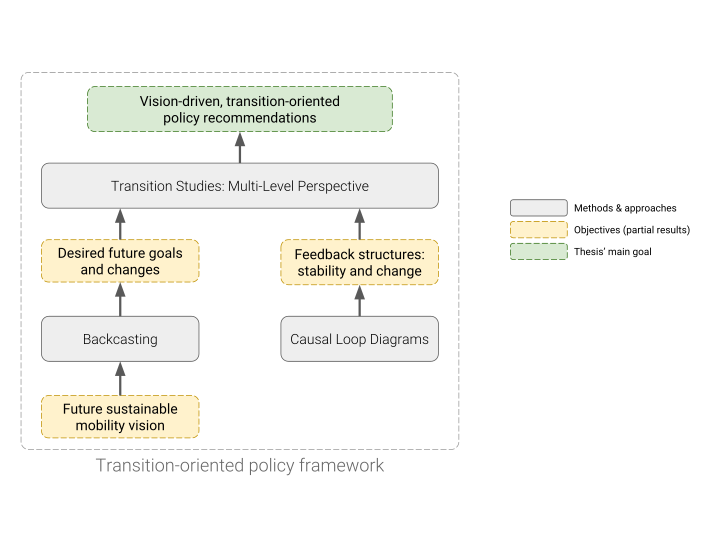
\includegraphics[width=\linewidth]{figures/methods-goals.pdf}
\caption[Thesis' methodological framework]{The generic methodological framework of the thesis. Note that the CLD model could be substituted by any other modelling technique which was sufficiently able to easily convey knowledge and insights to the key stakeholders and decision makers in the system.}
\label{f:thesis-aim-methods}
\end{figure}

\subsection{Backcasting}
\todoparagraph{Explain what backcasting is, what types are there (participatory, etc,) and why is it useful for the thesis (setting the final vision AND analysis of the changes/transition)}

\subsection{Causal Loop Diagrams}
\label{ss:methods:causal-loop-diagram-development}
\todoparagraph{Explain what CLDs are and how to read them. Provide the graphs from Sterman (chapter 4).}

\todoparagraph{Explain how the CLDs were developed: brainstorm + pruning, much like the planning framework described by \textcite{laurenti2015_TowardsAddressingUnintended} (Figure 5)}

\subsection{Transition theory}
\todonote{Rephrase this!}The combination of assessment and planning tools, embedded in the discourse of transition studies, is used to discuss possible global patterns of development, by means of a dual backcasting and forecasting approach: scenario backcasting on one hand and system dynamics modelling on the other.